Central Dogma of Molecular Biology
\[
\boxed{
    \begin{aligned}
        \text{DNA} \ &\xrightarrow{\text{transcription}} \text{mRNA} \xrightarrow{\text{translation}} \text{proteins}
    \end{aligned}
}
\]
Cells:\\
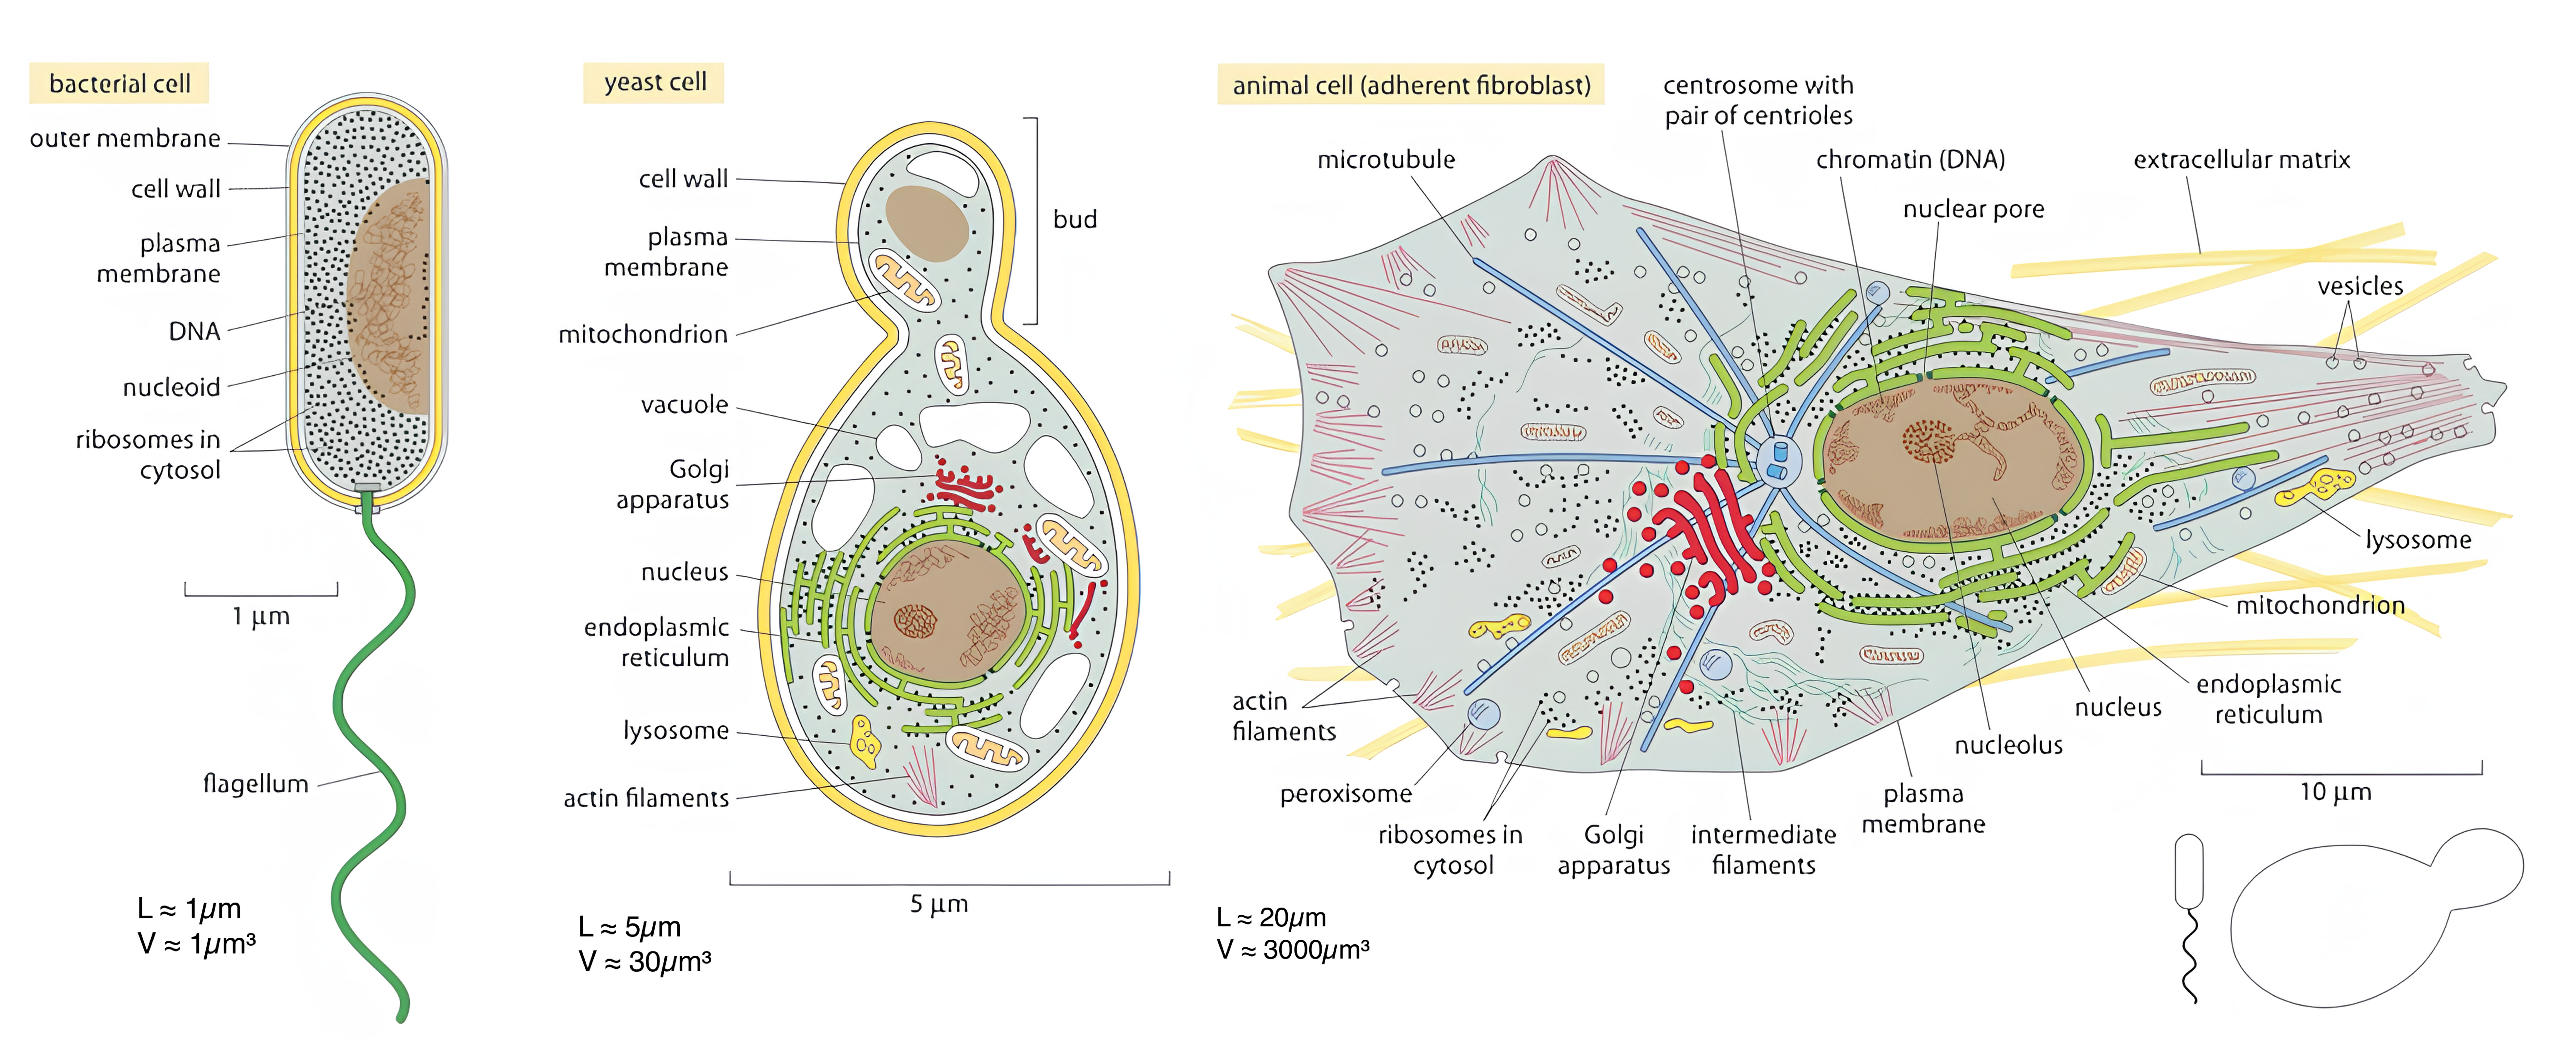
\includegraphics[width=7.3cm]{src/images/cell.png}

\begin{minipage}{0.45\linewidth}
    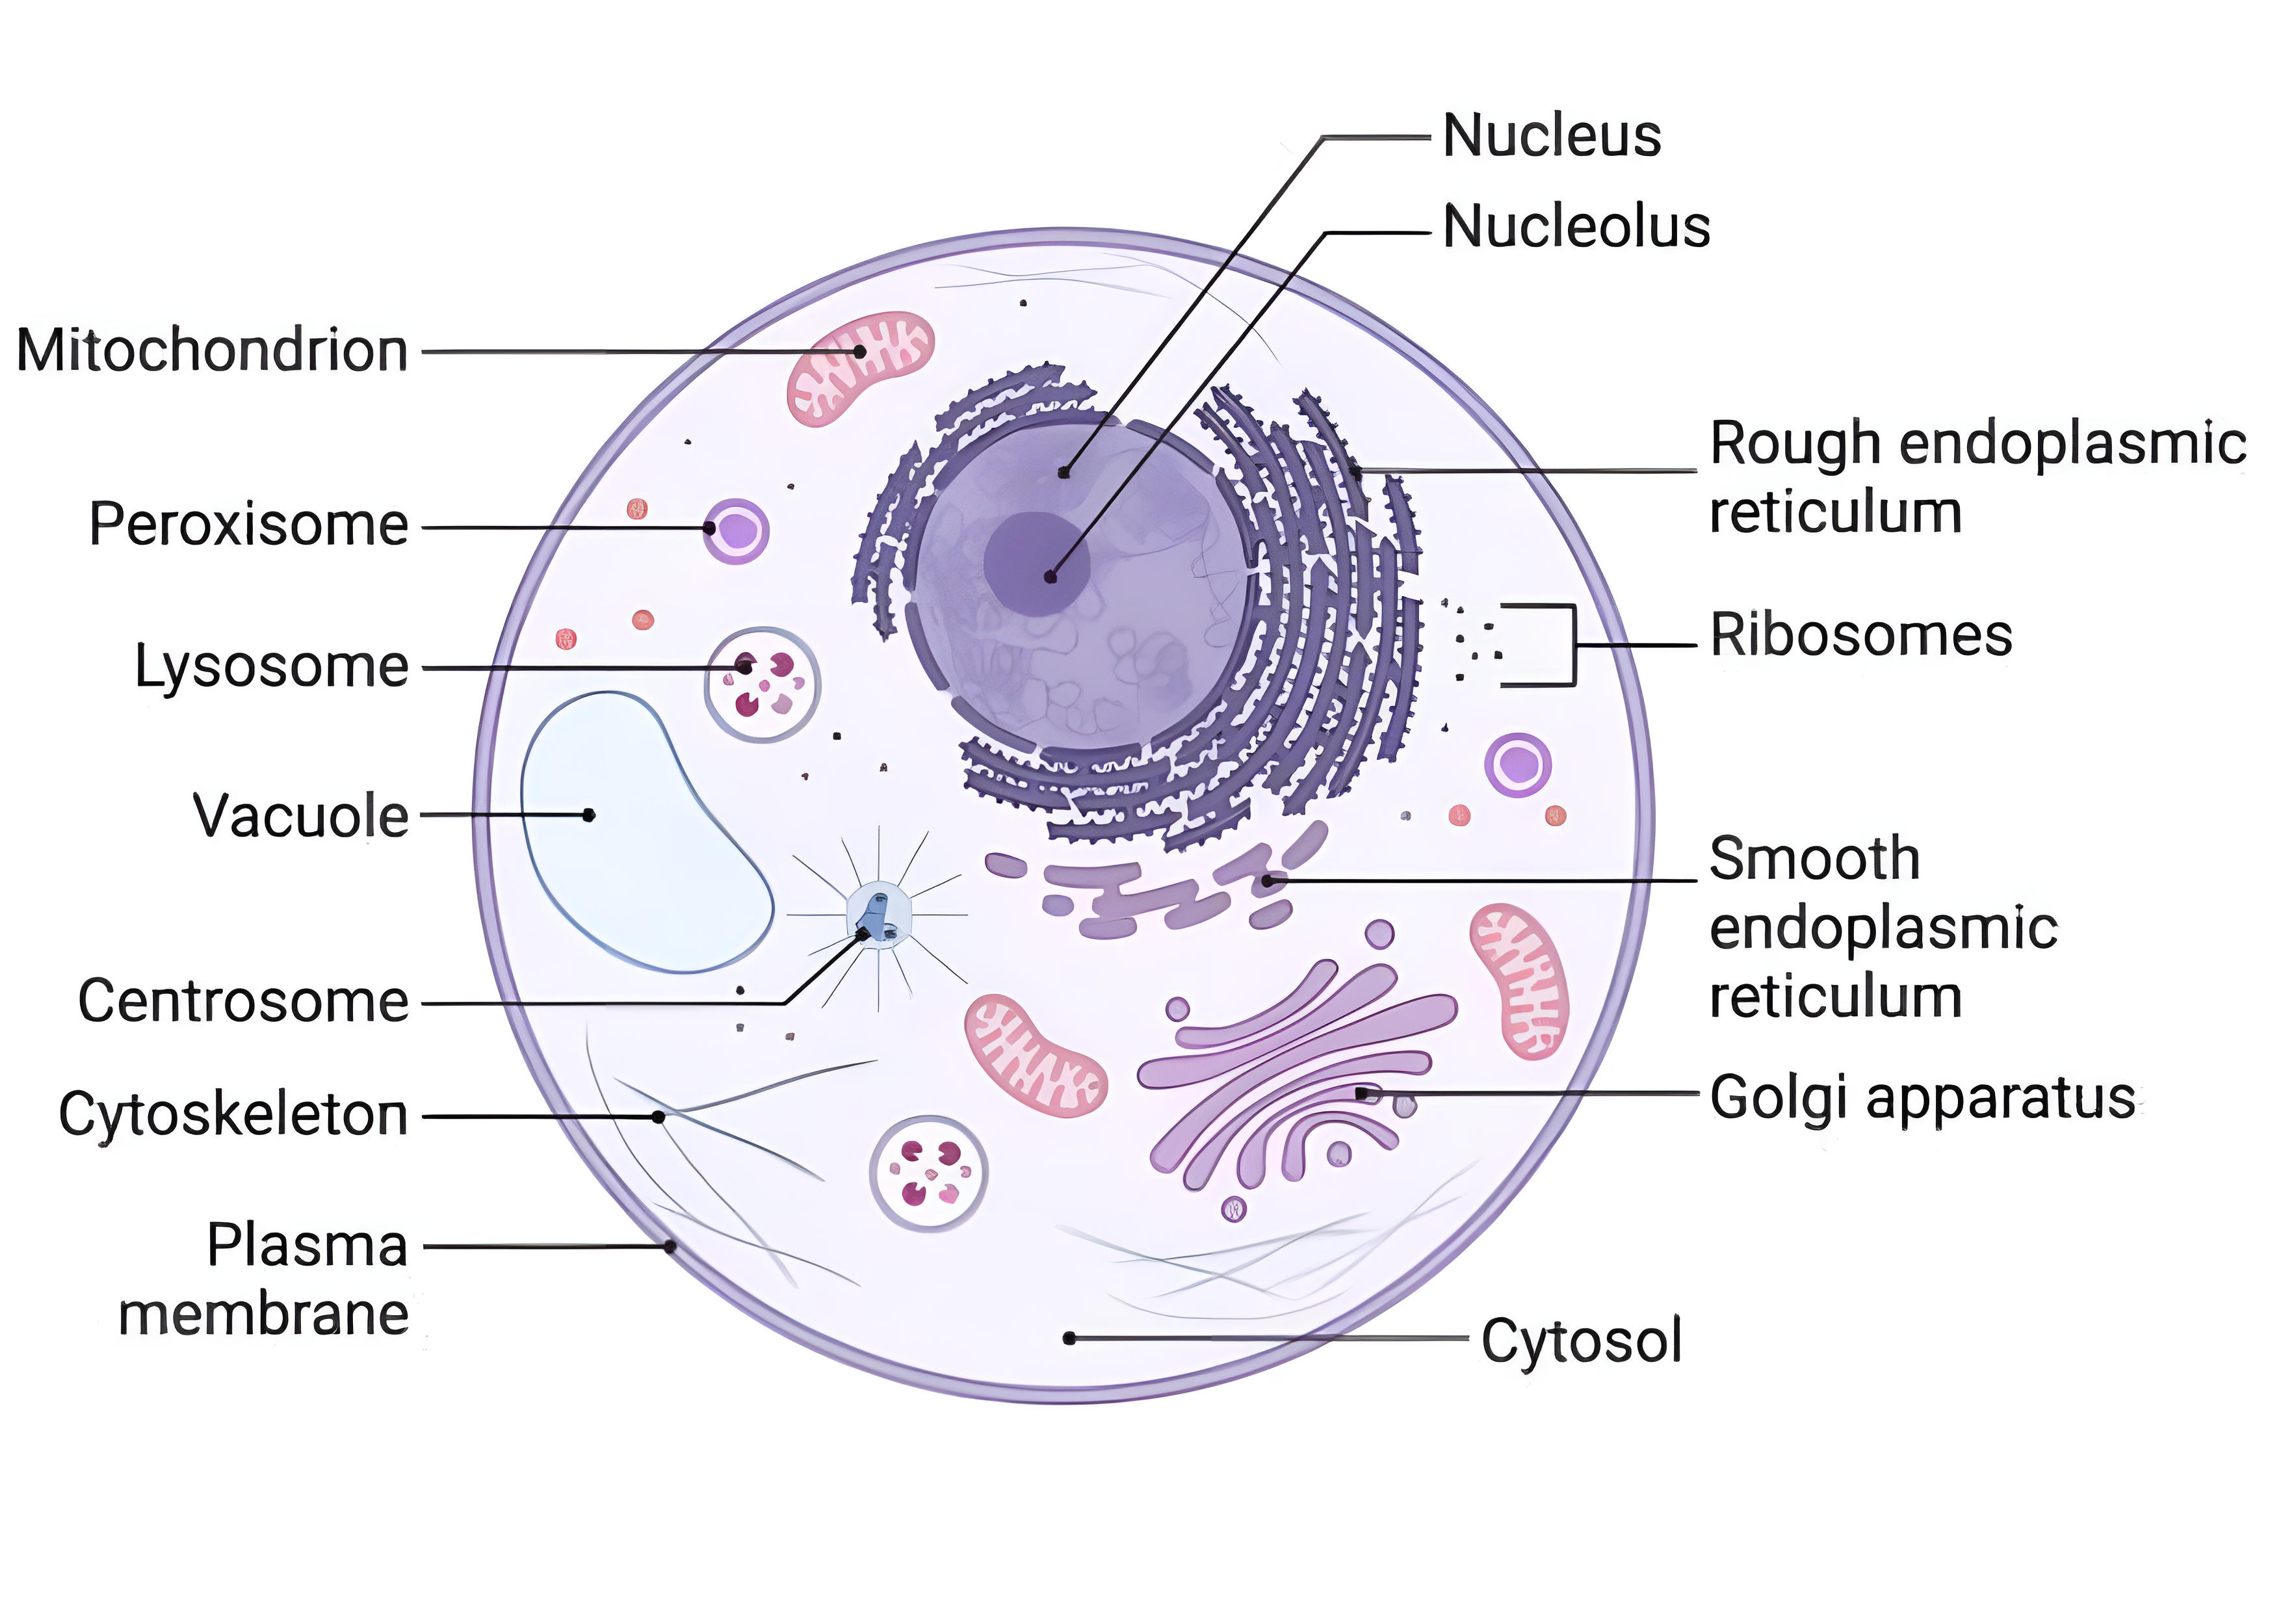
\includegraphics[width=3cm]{src/images/organelles.png}
\end{minipage}
\begin{minipage}{0.55\linewidth}
    \textbf{nucleus}: houses DNA for EK\\
    \textbf{nucleolus}: produces ribosomes/rRNA\\
    \textbf{mitochondria}: cellular respiration (prod. ATP)\\
    \textbf{ribosome}: produces proteins from mRNA transcripts\\
    
\end{minipage}
\vspace{1mm}
\textbf{RER, SER and Golgi}: involved in protein/lipid synthesis/processing\\
\textbf{cytoskeleton}: structure to cell, transport mol. in the cell or to enable the cell to move (cell migration)\\
\textbf{centrosome}: organizes microtubules during cell division allows the mother cell to split into 2 cells\\
